\paragraph{Modalità allenamento}

\subparagraph{Selezione parametri di set-up}

\label{Selezione parametri di set-up}

\begin{figure}[ht]
	\centering
	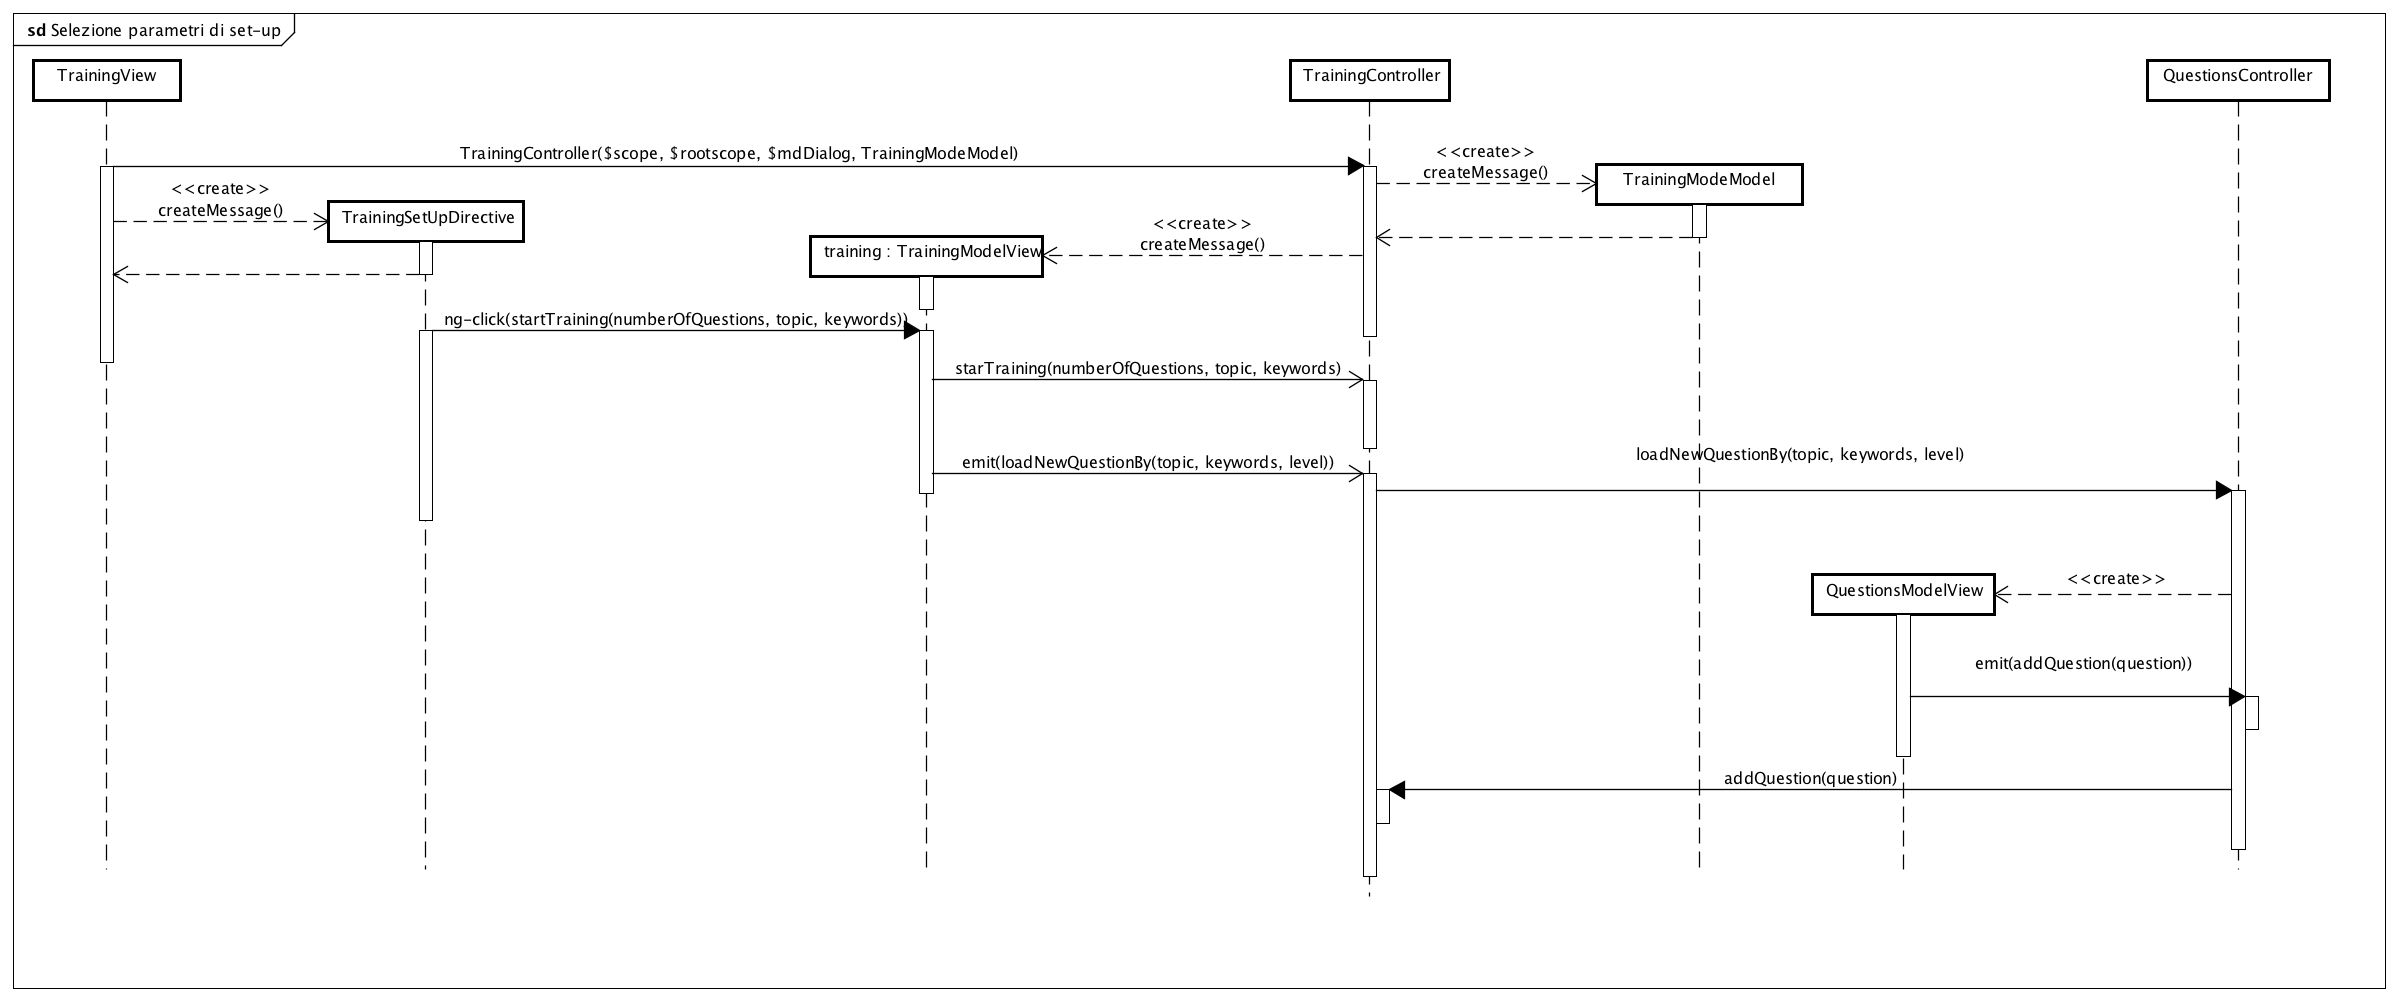
\includegraphics[scale=0.25,keepaspectratio]{UML/DiagrammiDiSequenza/Front-end/Training_setUp.png}
	\caption{Selezione parametri di set-up}
\end{figure} \FloatBarrier

Dopo che l'utente avrà selezionato i parametri per eseguire l'allenamento, cioè l'argomento, le parole chiave e il numero di domande l'allenamento avrà inizio. Se il numero di domande non viene indicato l'allenamento andrà avanti ad oltranza.

\subparagraph{Download di una domanda}

\label{Download di una domanda}

\begin{figure}[ht]
	\centering
	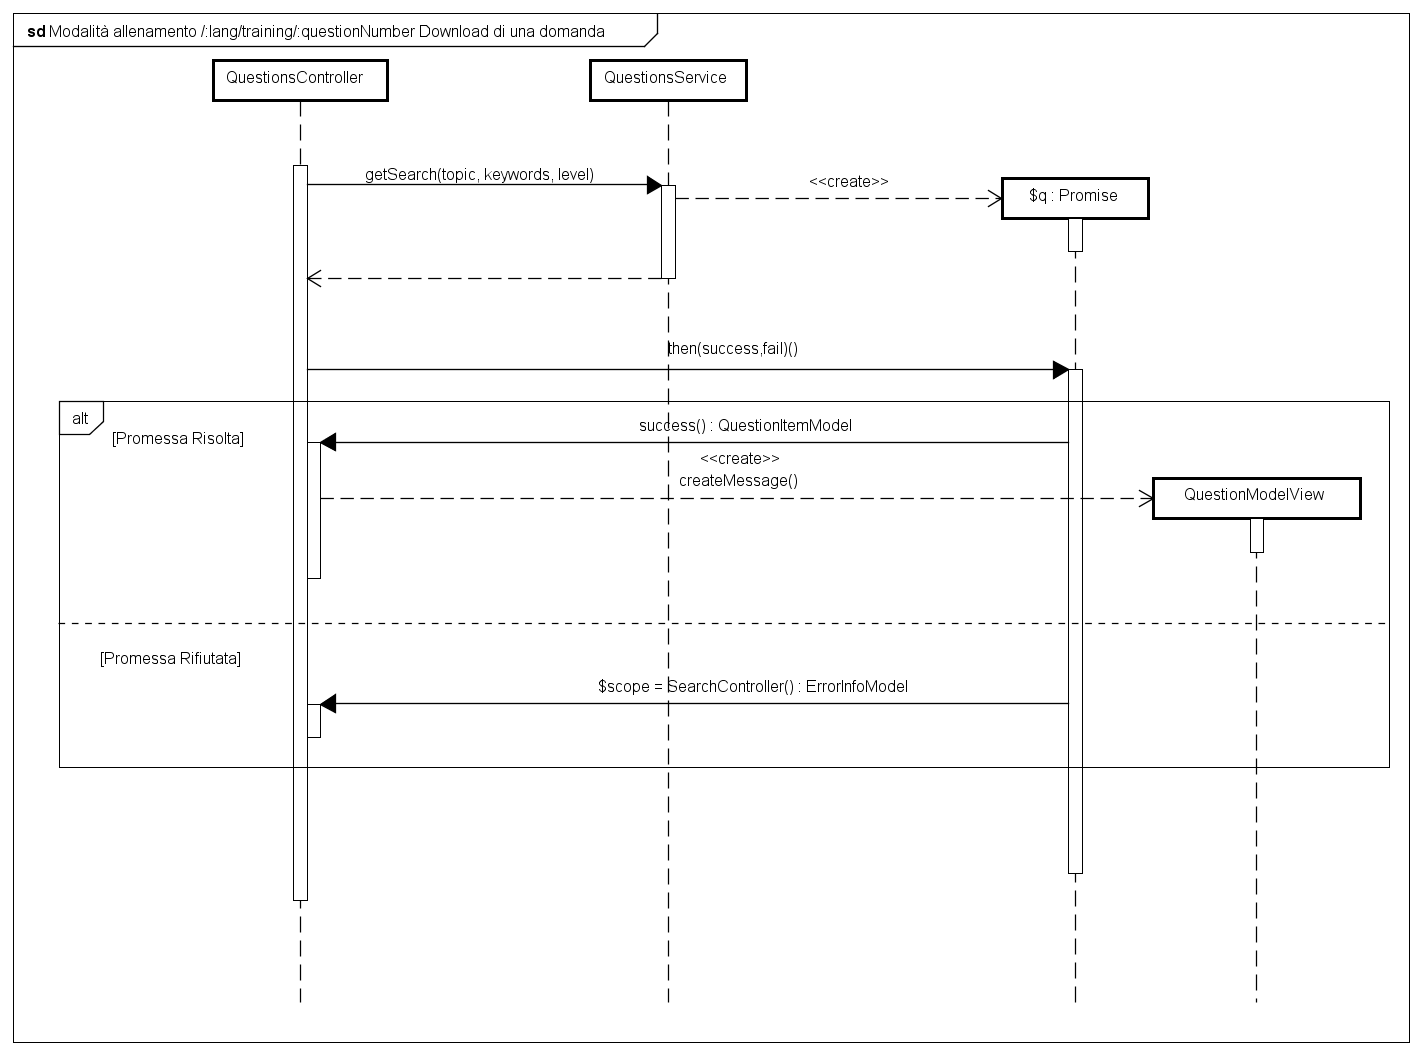
\includegraphics[scale=0.35,keepaspectratio]{UML/DiagrammiDiSequenza/Front-end/Training_downloadAquestion.png}
	\caption{Download di una domanda}
\end{figure} \FloatBarrier

Il \texttt{QuestionsService} restituisce a \texttt{QuestionsController} una promessa, se questa verrà rispettata verrà ritornato un oggetto di tipo \texttt{QuestionItemModel} altrimenti verrà restituito un oggetto di tipo \texttt{ErrorInfoModel} e mostrato a video mediante \texttt{\$mdDialog}.


\subparagraph{Composizione di una domanda}

\label{Composizione di una domanda}

\begin{figure}[ht]
	\centering
	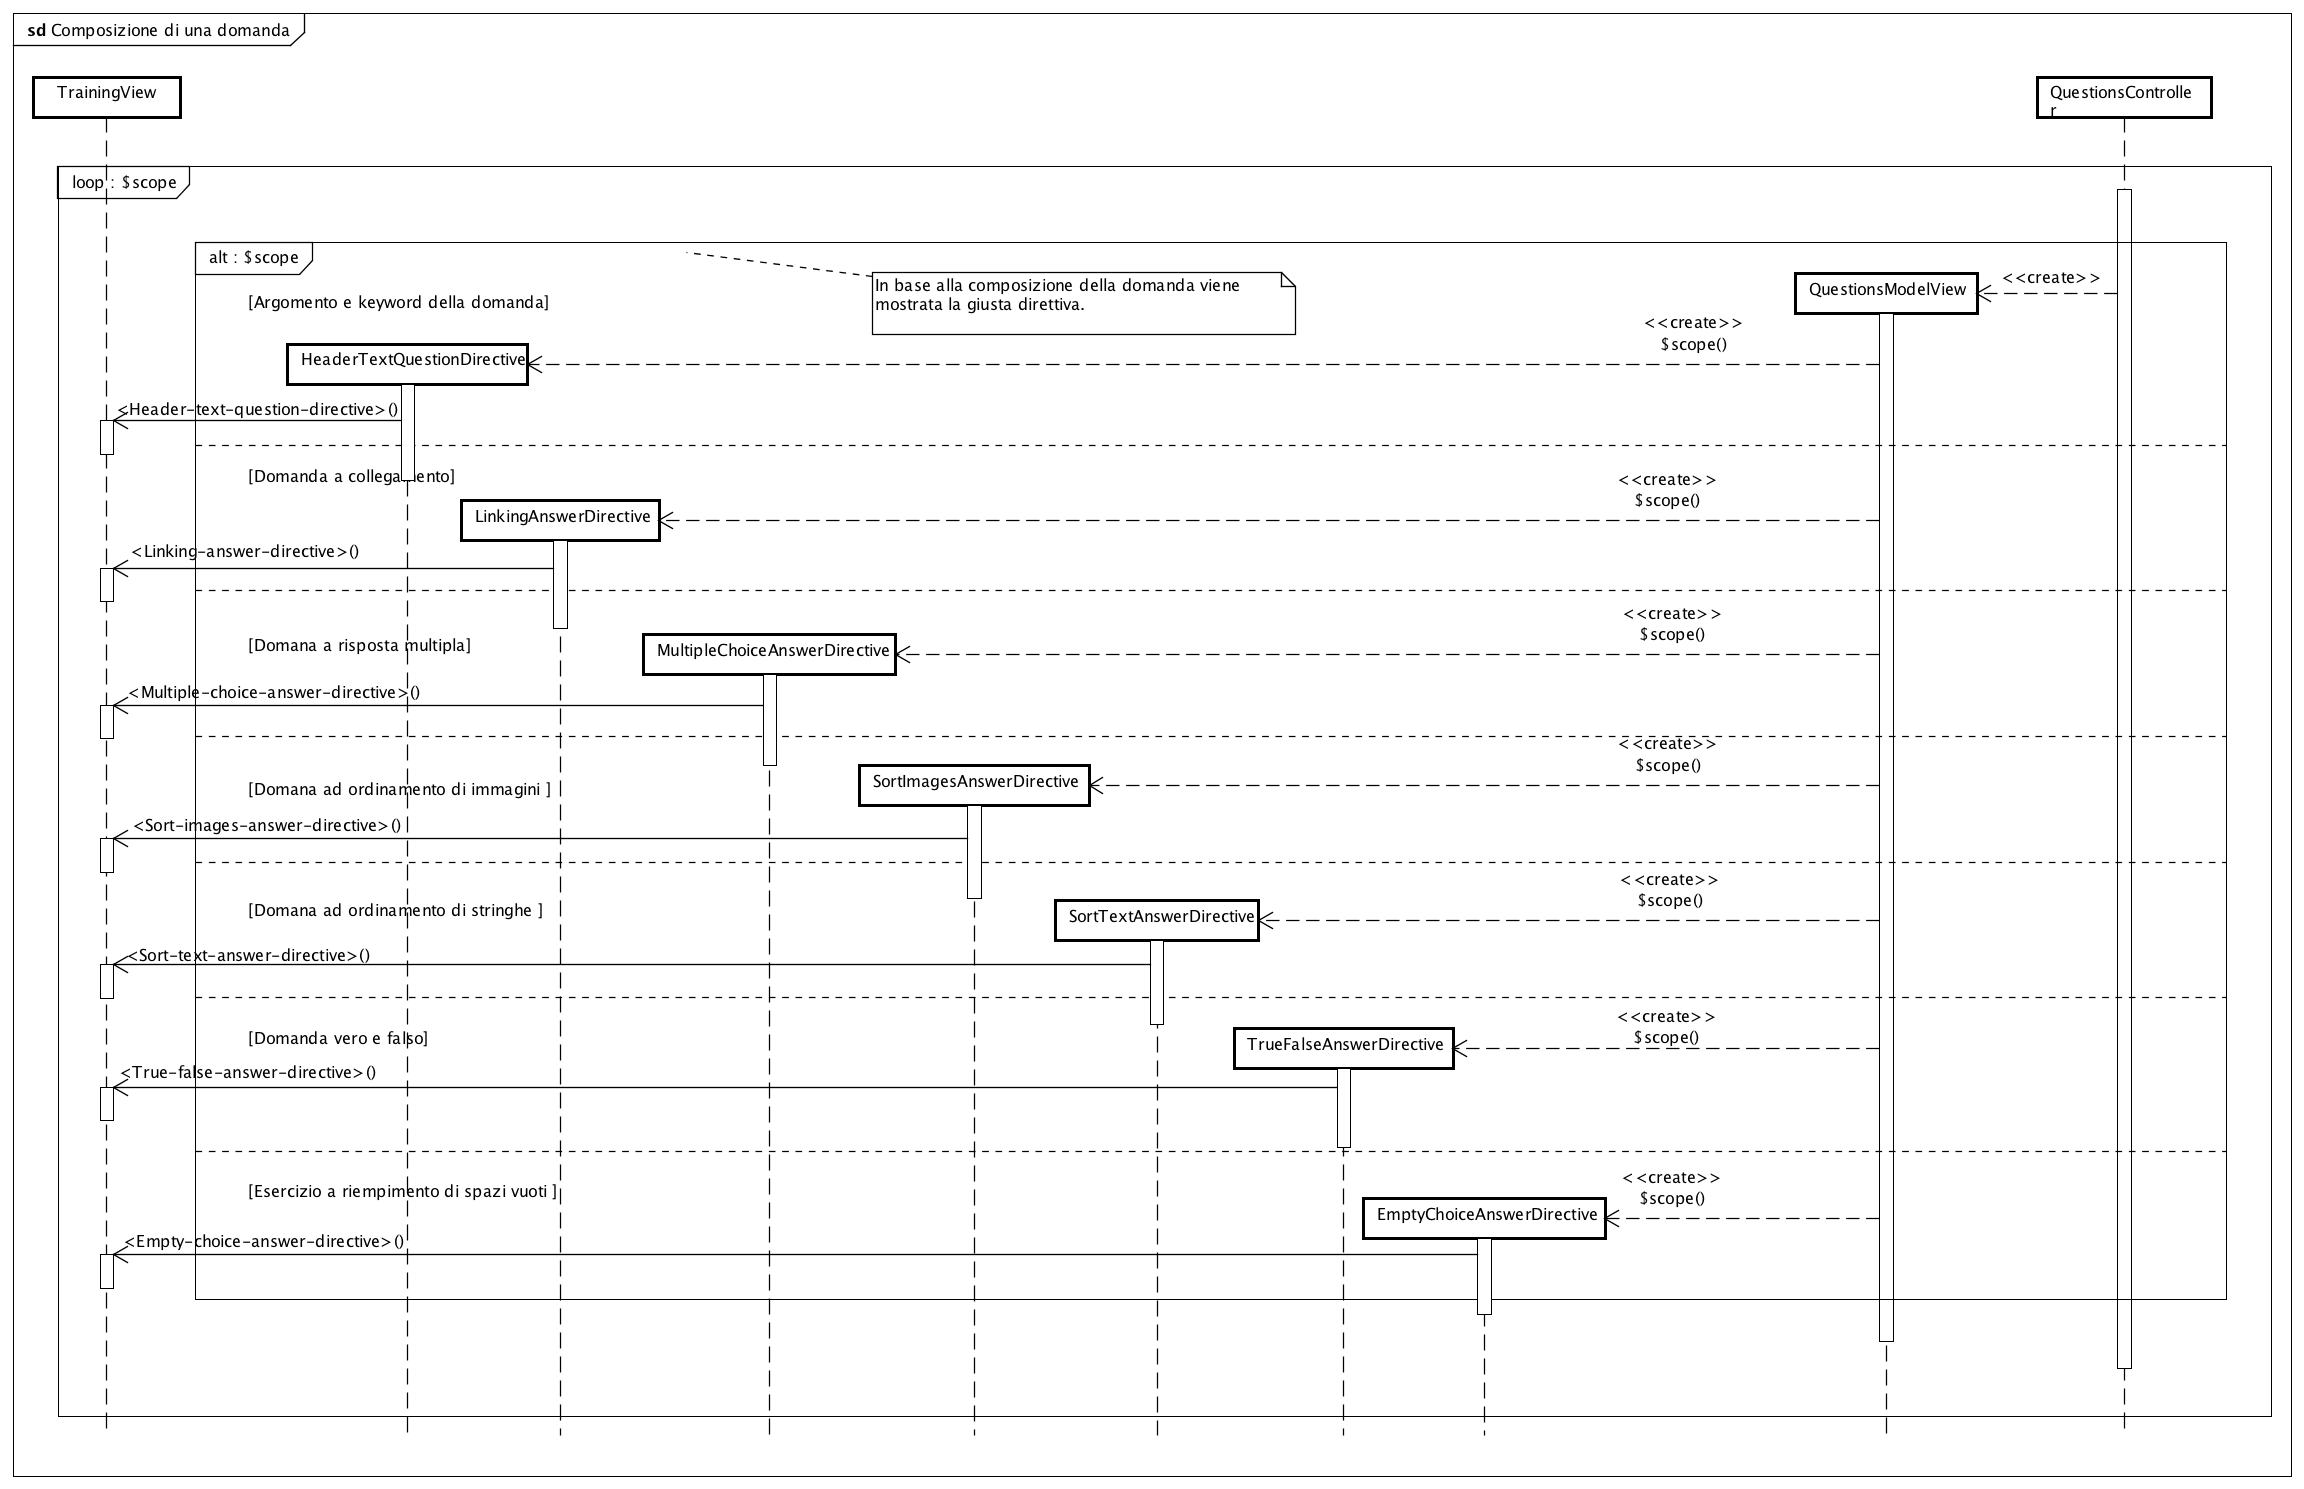
\includegraphics[scale=0.25,keepaspectratio]{UML/DiagrammiDiSequenza/Front-end/Training_makingAQuestion.png}
	\caption{Composizione di una domanda}
\end{figure} \FloatBarrier

Eseguendo un loop sulla variabile di tipo \texttt{QuestionsModelView} precisamente sull'array \\ \texttt{piecesOfQuestion}, per ogni pezzo di domanda verrà visualizzata la giusta direttiva così da comporre la domanda nella sua totalità.

\subparagraph{Risposta ad una domanda}

\label{Risposta ad una domanda}

\begin{figure}[ht]
	\centering
	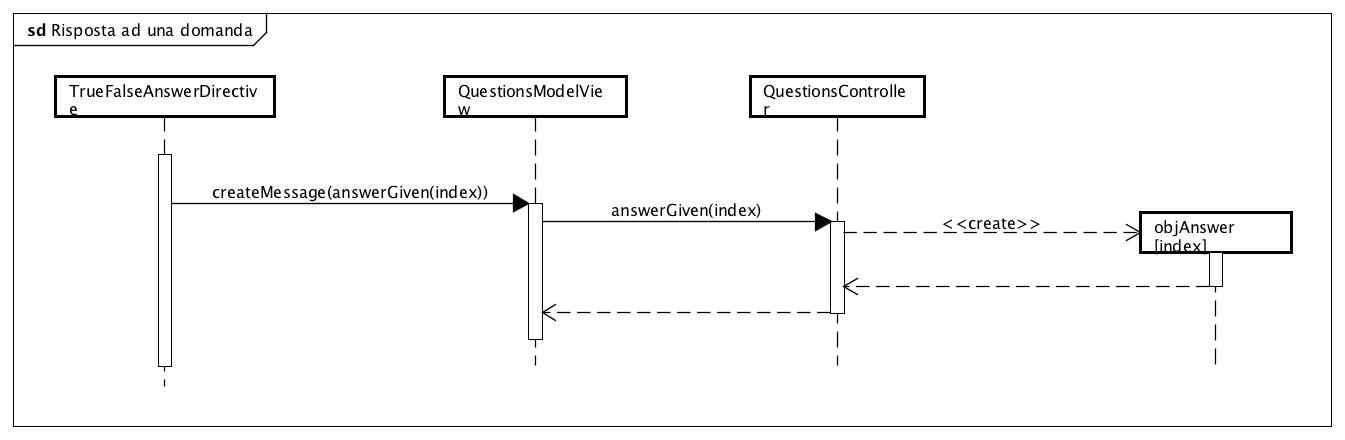
\includegraphics[scale=0.4,keepaspectratio]{UML/DiagrammiDiSequenza/Front-end/Training_answerAQuestion.png}
	\caption{Risposta ad una domanda}
\end{figure} \FloatBarrier

In questo diagramma di sequenza viene mostrato come avviene la selezione di una riposta vero/falso. Il procedimento è uguale per tutte le tipologie di domande. Ad ogni evento \texttt{ng-change} o \texttt{ng-click} viene aggiornato l'oggetto \textbf{objAnswer} nella giusta posizione. Alla conclusione della risposta l'oggetto \texttt{objAnswer} conterraà tutte le risposte date per quella domanda. 
